\subsection{Magnetisation pools}
\label{subsec:noah__magpools}

Having gotten this relatively dry material out of the way, I now turn to exactly how NOAH supersequences are constructed.
Ordinarily, if the recovery delay is removed from an NMR experiment, its sensitivity will be greatly reduced because insufficient magnetisation will have recovered between repetitions; or in other words, $A^{(i)}$ will be very small.
Such experiments would only really be useful well in the sampling-limited regime.

The key to avoiding this in NOAH supersequences is to make sure that \textit{each module samples a different source of magnetisation}.
For example, a HSQC module can be designed to only sample magnetisation of protons directly bonded to the 1.1\%-natural abundance \carbon{}, and leave all other proton magnetisation untouched.
Immediately following this, the remainder of the proton magnetisation can then be used to record (say) a COSY module, without needing a separate recovery delay.
Using the notation of Orts and Gossert\autocite{Orts2018M}, the magnetisation of \carbon{}--bound protons is denoted as \magn{C}, and the magnetisation of protons \textit{not} bonded to \carbon{} is denoted as \magnnot{C}.
Protons not directly bonded to NMR-active heteronuclei are labelled \magnnot{X}, and will often be referred to as `bulk' magnetisation, since (in natural-abundance samples) the majority of protons fall into this category.

Most standard 2D experiments do not preserve unused magnetisation but instead dephase it through CTP gradient selection; thus, NOAH modules often require some modifications compared to standard experiments.
For example, compared to the echo--antiecho HSQC (discussed in \cref{subsec:theory__hsqc_ea}), the NOAH HSQC module\autocite{Kupce2017ACIE} adds an extra CTP gradient so that the bulk magnetisation is refocused and ultimately returned to the $+z$ equilibrium state (\cref{fig:noah_hsqc}).
(This is largely identical to the `symmetrised' ASAP-HSQC experiment\autocite{SchulzeSunninghausen2017JMR}.)

\begin{figure}[htb]
    \centering
    \includegraphics[draft=false]{pp/hsqc/noah_po}%
    \caption[NOAH HSQC module with product operator analysis]{
        NOAH HSQC module.
        The delay $\Delta$ is set to $1 / (4 \cdot \oneJ{CH})$.
        Phase cycling is performed with $\phi_1 = (x, -x)$, $\phi_2 = (x, x, -x, -x)$, and $\phi_\text{rec} = (x, -x, -x, x)$.
        Gradient amplitudes are $(g_1, g_2) = (80\%, \pm 40.2\%)$.
        The notation for product operator analysis is explained in the \textit{Preface}.
    }
    \label{fig:noah_hsqc}
\end{figure}

Sometimes, the modifications required are more extensive, as in the HMBC module.
If this module is followed by a HSQC module (or any other module which draws on \magn{C} magnetisation), the initial \ang{90} excitation pulse must be replaced with a $zz$-filter (\cref{fig:noah_hmbc_no90_po}).
This performs an \textit{isotope-selective rotation} in that \magn{C} magnetisation is stored along the $z$-axis, but \magnnot{C} magnetisation is excited (and subsequently detected).
In general, sequences which are thus modified have lower sensitivities (i.e.\ $A < 1$) than the `original' sequences from which they were derived.

\begin{figure}[htb]
    \centering
    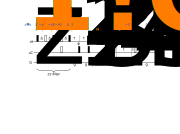
\includegraphics[draft=false]{pp/hmbc/noah_no90_po.png}%
    \caption[NOAH HMBC module with product operator analysis]{
        NOAH HMBC module.
    Delays are set as: $\Delta = 1 / (2 \cdot \nJ{CH})$; $\tau_1 = 1 / (2 \cdot \oneJ{CH,\text{max}})$; $\tau_2 = 1 / (2 \cdot \oneJ{CH,\text{min}})$ (see also \cref{subsec:poise__hmbc}).
        Phase cycling is performed with $\phi_1 = (x, -x)$, $\phi_2 = (x, x, -x, -x)$, and $\phi_\text{rec} = (x, -x, -x, x)$.
        Gradient amplitudes are $(g_1, g_2, g_3, g_4, g_5) = (15\%, -10\%, -5\%, 80\%, \pm40.2\%)$.
    }
    \label{fig:noah_hmbc_no90_po}
\end{figure}

In contrast, modules placed towards the \textit{end} of a supersequence do not need to be modified, as they do not need to preserve any magnetisation.
This includes virtually all homonuclear modules, which are allowed to simply consume any remaining magnetisation.
Although this makes their implementation very straightforward, in general these modules will \textit{also} suffer some losses in sensitivity, because the preceding modules do not perfectly retain all magnetisation.

Thus, in general, it is not possible for any module in a NOAH supersequence to have $A = 1$, unless it is placed first in the supersequence \textit{and} has not undergone any modifications.%
\footnote{Of course, this also depends on exactly \textit{what} standalone experiment the NOAH supersequence is being compared against. Sometimes, in the literature, the NOAH experiment has been compared against its constituent modules acquired in a standalone fashion; in this case, the first module will always have $A = 1$. This tells us how much we gain through the act of concatenating modules, but is less meaningful in the `real world' where one is interested in how useful NOAH is relative to `typical' optimised 2D experiments. I therefore prefer to make comparisons against standard-library sequences.}
Such cases are very rare, and it is thus necessary to accept some decreases in $A$, which are often fairly small (on the order of 10--20\%).
In the sampling-limited regime, sensitivity is not at a premium and this is often perfectly tolerable.
In the sensitivity-limited regime, the full time savings $\rho_t$ cannot be realised, but since $\varepsilon$ is still typically larger than 1, there is still an overall boost in sensitivity per unit time.
